\documentclass{article}
\usepackage{pdfpages,listings,graphicx,hyperref}
\usepackage[export]{adjustbox}
\hypersetup{
	colorlinks=true,
	linkcolor=blue
}
\title{Solving the Windy GridWorld with SARSA}
\author{George Fakidis, Athens University of Economics and Business}

\begin{document}
\maketitle

\section{Code}
The full code can be found in \href{https://github.com/GeorgeFkd/aueb-cs-masters/blob/master/reinforcement-learning/RL-hw6.py}{My Github}.

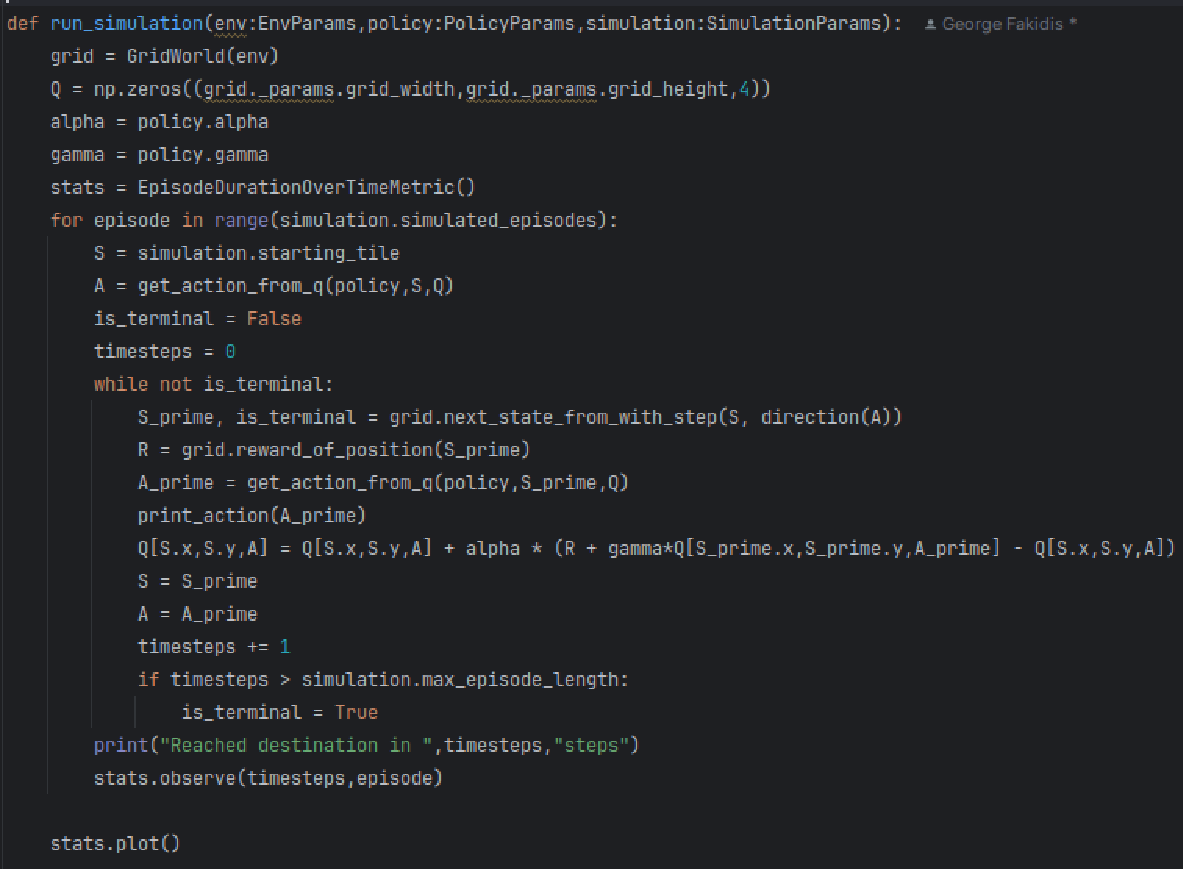
\includegraphics[scale=0.9,center]{img.pdf}

Implementation details regarding the GridWorld and the policy were left out intentionally in order to focus on the SARSA algorithm.
\section{Charts}
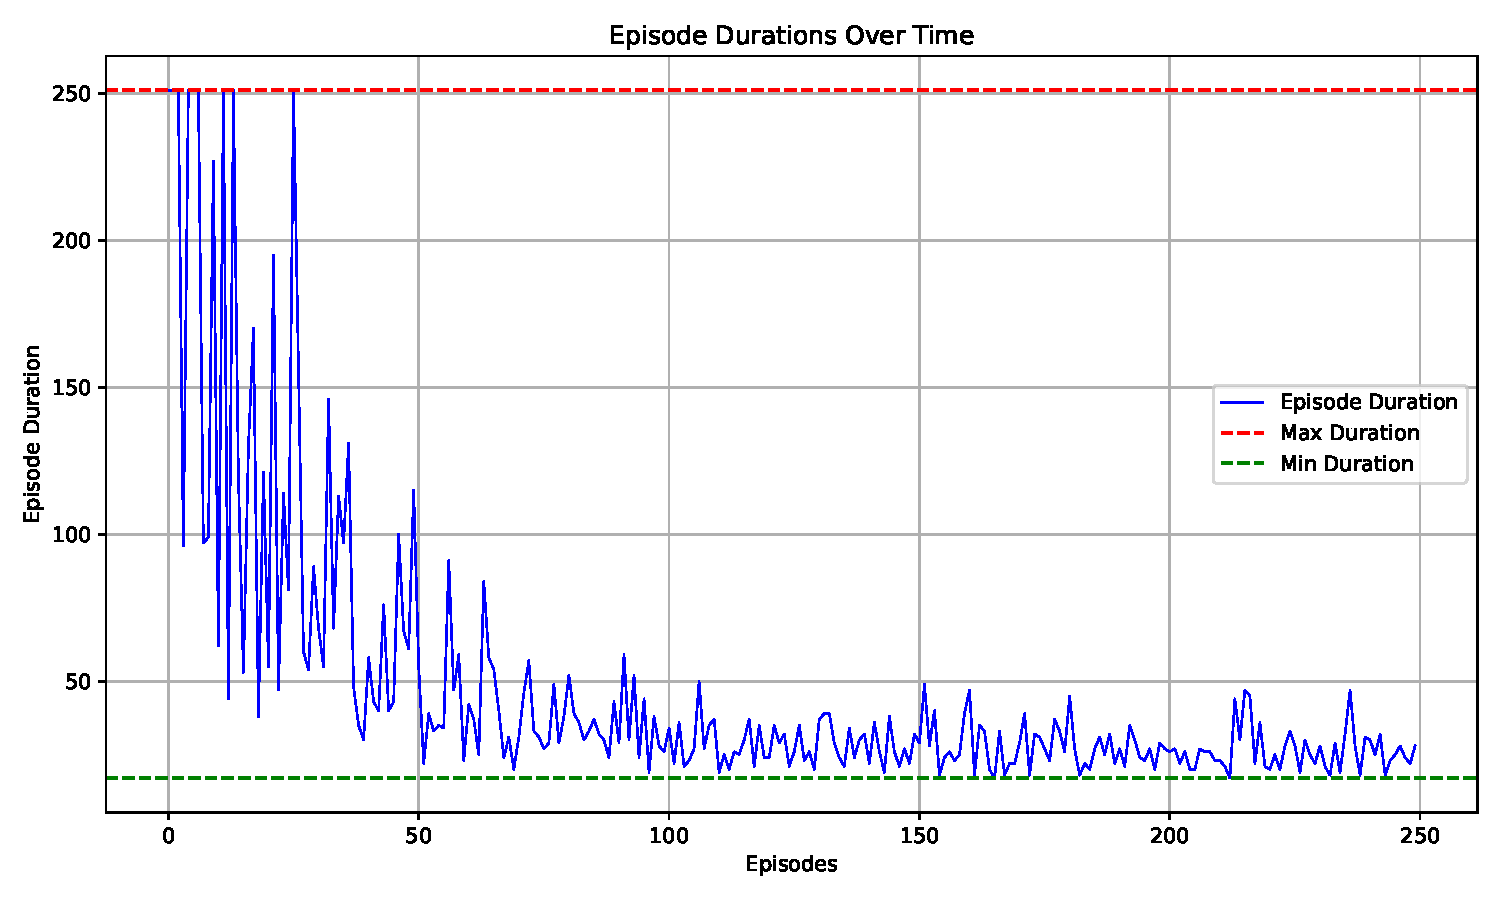
\includegraphics[scale=0.8,center]{Windy Grid World with SARSA.pdf}
\par
This is how the algorithm behaves, the main thing to notice here is that episodes
last less as time progresses, meaning our algorithm actually learns how to navigate
the windy landscape.

\end{document}
